% ============================================================================================
% PAPER 1, LONG FORMAT (PRE / Soft Matter / PRX-length): skeleton with drafted lead paragraphs. Started 2026-10-14.
% Scope (user, 2026-10-13): cavities only; channels only as the flat limit of the wall law (Sec. VIII D).
% Strategy: the long version carries the full mechanism (escape dynamics, steady state, wall law) that the PRL can only summarise.
% Each section: lead paragraph drafted in paper register + "%% CONTENT" list of the results to write out, with the source in the
% theory report (reports/theory_report) and the figure plan. Numbers: theory report 2026-10-14 and RESEARCH.md.
% ============================================================================================
\documentclass[aps,pre,twocolumn,superscriptaddress,amsmath,amssymb,reprint]{revtex4-2}
\usepackage{graphicx}
\usepackage{xcolor}
\usepackage[hidelinks]{hyperref}
\graphicspath{{../../theory_report/figs/}}
\DeclareGraphicsExtensions{.pdf,.png}
\newcommand{\half}{\tfrac12}
\newcommand{\la}{\ell_a}
\newcommand{\kT}{k_BT}
\newcommand{\todo}[1]{\textcolor{red}{[TODO: #1]}}

\begin{document}

\title{Overcharged active nematic cavities: flow-induced ejection, a flow-aligned tilt law, and how elongated layers leak}
\author{Benjamin Loewe}
\affiliation{Facultad de F\'isica, Pontificia Universidad Cat\'olica de Chile, Santiago 7820436, Chile}
\author{Tyler N. Shendruk}
\affiliation{School of Physics and Astronomy, The University of Edinburgh, Peter Guthrie Tait Road, Edinburgh EH9 3FD, United Kingdom}
\date{\today}

\begin{abstract}
\todo{~250 words. Same arc as the PRL abstract, plus: the escape mechanism (jet blocked by the no-slip wall, wall-side lobe erased, untilting runaway, landing on
viscometric lines), the steady state as a unique dynamical balance limited by layer crowding, and the wall law with its channel limit.}
\end{abstract}
\maketitle

% ============================================================================================
\section{Introduction}\label{sec:intro}
%% CONTENT: confined active nematics (coherent vortices, channels \cite{Shendruk2017}); anchoring fixes the topological charge; patterned winding;
%% prior work on imposed net charge: active flow screens the anchoring, dynamics insensitive to the topological constraint \cite{Norton2018}; overcharged disks
%% with periodic defect orbits \cite{Klein2026}; confined active nematics in disks and channels \cite{Opathalage2019,Hardouin2019,Hardouin2022}; active suspensions in circles
%% and racetracks \cite{Theillard2017}; what is new here: mechanism, tilt law, escape physics, wall law; links to viscometric constraints \cite{Head2024}.
%% TODO(Benjamin): framing.
\todo{introduction}

% ============================================================================================
\section{Model and observables}\label{sec:model}
We simulate a two-dimensional active nematic with multi-particle collision dynamics (MPCD) in the NIAMH-MPCD implementation \cite{Kozhukhov2022}. Lengths are
in collision cells, times in MPCD time units (t.u.), energies in $\kT$; the mean density is 20 particles per cell. Extensile active dipoles with activity
$\zeta=0.07$ set the active length $\la=22.2\pm0.3$ cells \cite{Kozhukhov2024}. \todo{collision operator, nematic mean field, flow alignment $\lambda$ (Jeffery/Bretherton), wall
collisions, anchoring $\theta=k\phi$ uniform in arclength; Frank constants and rotational viscosity measured (SM)}
%% CONTENT: cavities (circles R/l_a 0.2-2.9, k 2-10; ellipses eps 1.2-2.5; Cassini ovals; R_eq = sqrt(area/pi) = 1-2 l_a; 675 shape runs, 3 seeds; circles: 10 seeds, 510 runs in the window);
%% defect tracking and the head/tail convention (angle = direction of div Q = tail); wall layer = +1/2 within 4 cells (justified in App. B, layer profile);
%% observables: wall count, bulk charge Q_b, tilt tau_j, tilt coherence C = |<e^{i tau_j}>|, circulation, two-vortex fraction; escape / depleting escape; control defects.
%% Continuum models: passive Q-tensor with imposed flow; active Q-tensor with Stokes backflow; flat-wall model (App. A).

% ============================================================================================
\section{Overcharged circles}\label{sec:circles}
In passive cavities all $2k$ $+\half$ defects sit in a ring at the wall. With activity and $0.8\lesssim R/\la\lesssim2.2$ the wall holds exactly $2k-2$ defects and the bulk a
net charge $+1$, while $\pm\half$ pairs are created and annihilated in the bulk; one vortex fills the cavity and the wall defects tilt by 61--66$^\circ$ (low wall density) in its sense.
%% CONTENT: Fig. maps_circles; wall count and bulk charge vs R/l_a and k (server sweep, 10 seeds); onset of tilt/circulation R/l_a ~ 0.4-0.6 (effective-boundary stability, Sec. VI); full layer + bulk +1 for 0.8 <= R/l_a <= 2.2;
%% wall exchange ('duck-duck-goose'): an entry triggers a non-local exit; vacancy field ~140 kBT spans the cavity and points at the hole (Fig. fig_vacancy_field);
%% half-integer k (odd layers); negative winding (MPCD 13.5 of 14 predicted in the circle, 13.0 at aspect 2; seeded starts) -> open point, discussion.
\begin{figure}[t]
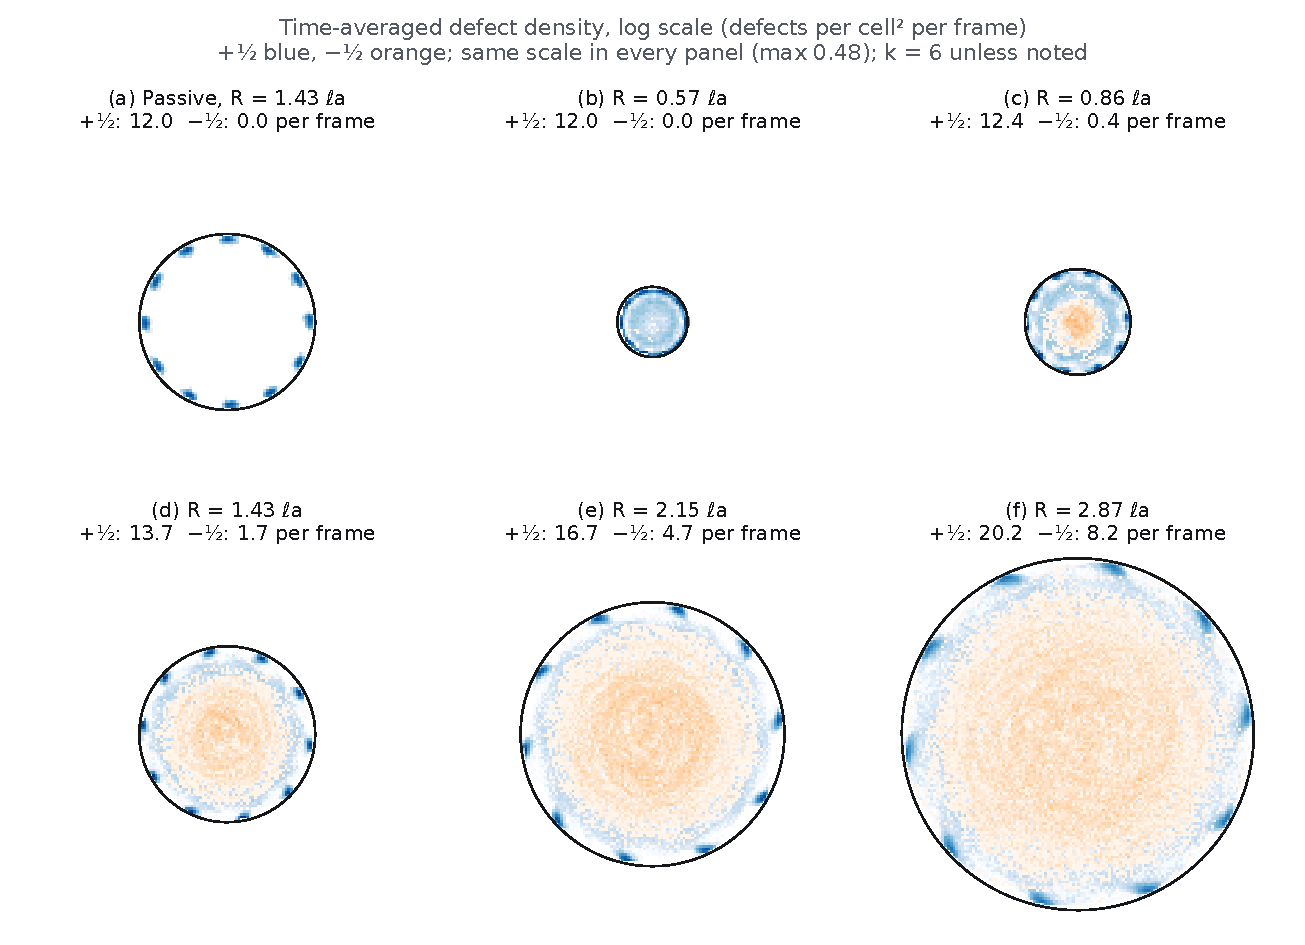
\includegraphics[width=\columnwidth]{maps_circles}
\caption{\todo{Fig.~1}: defect density maps, passive and active at increasing $R/\la$ ($k=6$).}\label{fig:maps}
\end{figure}

% ============================================================================================
\section{Anchoring geometry: sites, the tilt--position lock and pinning}\label{sec:lock}
Relative to the local wall normal the anchored director turns by $(k-1)\phi$, so it is homeotropic at $2k-2$ points, and the tilt of a wall $+\half$ is locked to
its position, $\tau_j=(2k-2)\phi_j+\text{const}$.
%% CONTENT: (2k-2)-fold symmetry; lock (resultant 0.99; local version in every shape 0.91-0.99); commensurability (2k ring tilts wind twice, measured -60 deg steps);
%% pinning needs K1 != K3 (barrier 80-110 kBT; passive 2k ring < 1 kBT, registry set by the initial condition; modulated winding test);
%% fluctuations (Hessian theory within 2-4 %). Fig. fig_lock.
\begin{figure}[t]
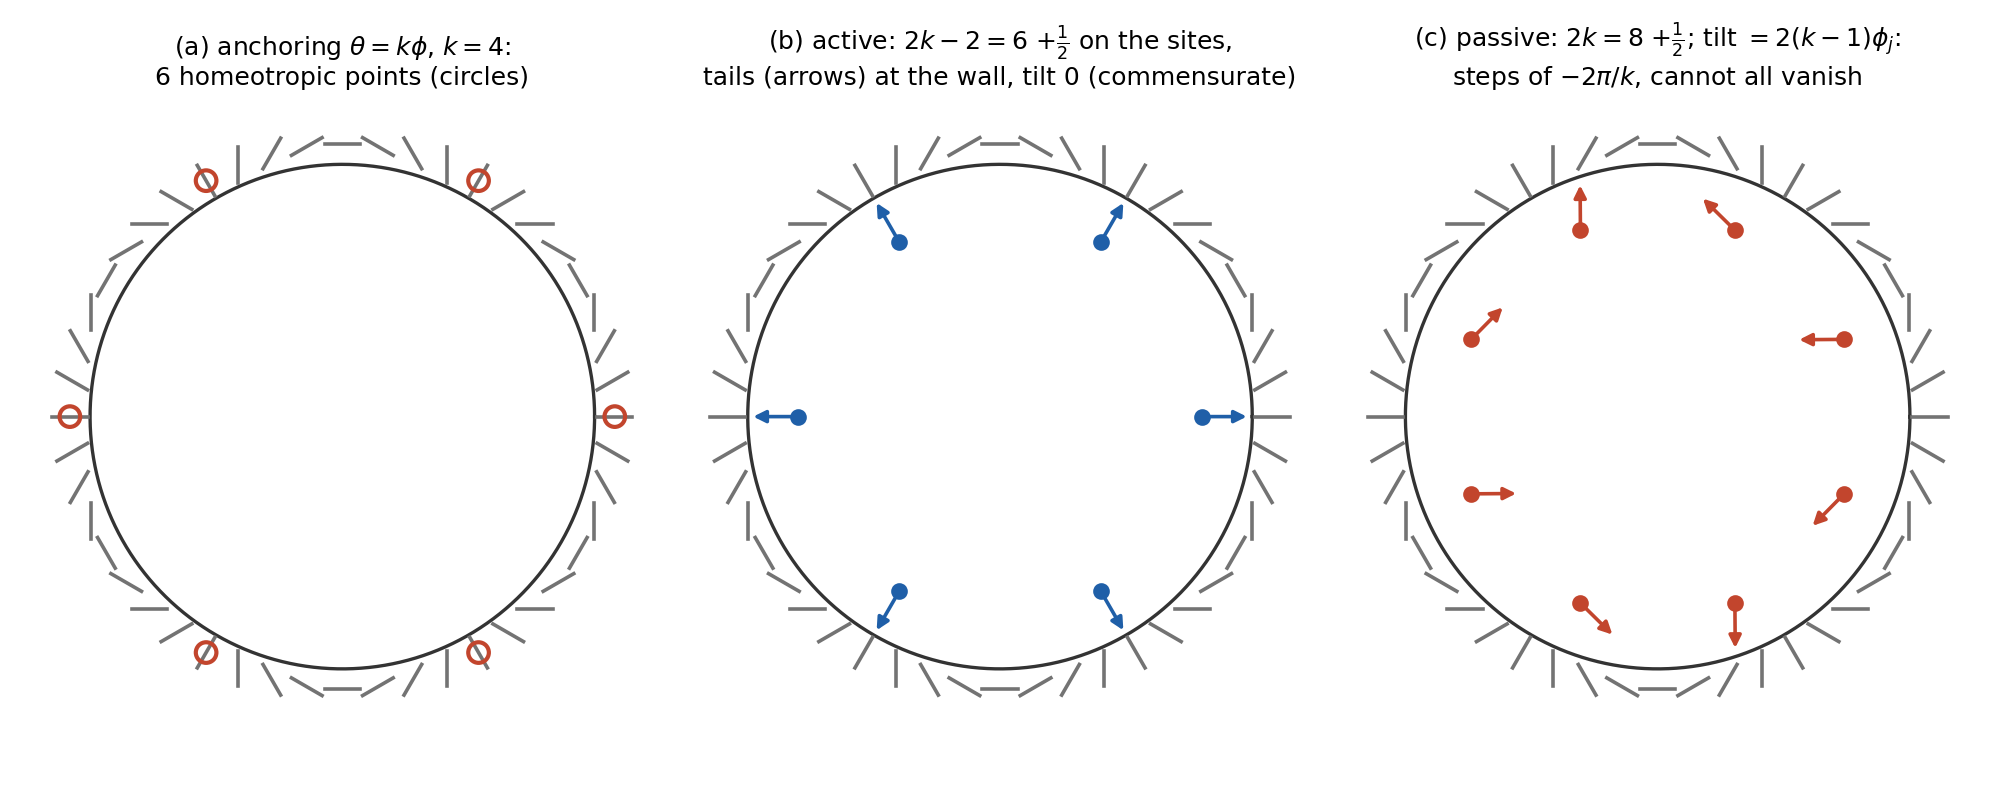
\includegraphics[width=\columnwidth]{fig_lock}
\caption{\todo{Fig.~2}: anchoring sites and the tilt--position lock ($k=4$).}\label{fig:lock}
\end{figure}

% ============================================================================================
\section{Flow-induced ejection}\label{sec:ejection}
A coherent flow imposes a common tilt on the wall layer. By the lock this is free for a ring of $2k-2$ and frustrating for a ring of $2k$, which ejects two defects.
%% CONTENT: energetics (Fig. tilted_structures: common tilt costs the 2k ring 375-475 kBT at k=6 (200-510 for k=4-8) vs 180-200 (155-200) to eject; one-constant and anisotropic);
%% passive cavity + imposed vortex (Fig. fig_ejection: threshold, needs common tilt C > 0.9, needs flow alignment; tumbling never);
%% continuum: passive Q-tensor with the measured flow (no fit) and active Q-tensor with backflow (one vortex, 2k-2, bulk +1).
\begin{figure}[t]
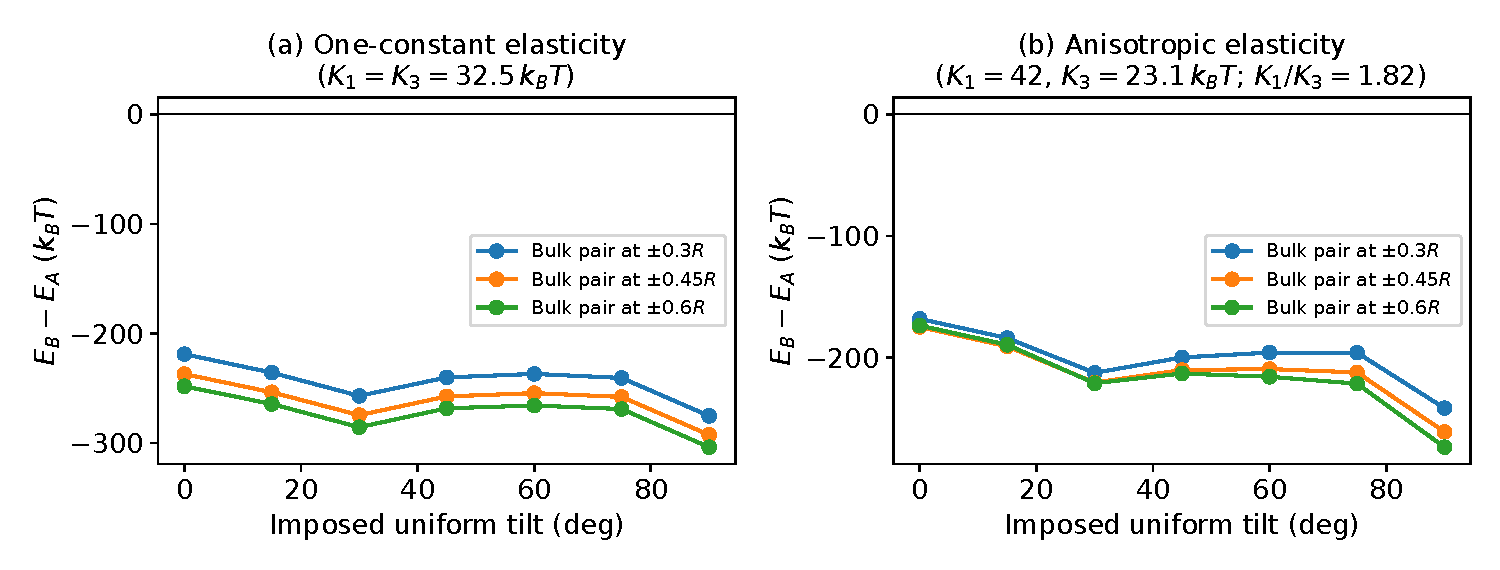
\includegraphics[width=\columnwidth]{tilted_structures}
\caption{\todo{Fig.~3}: energetics of ejection under a common tilt; with Fig.~\ref{fig:ejection} (imposed vortex).}\label{fig:energy}
\end{figure}
\begin{figure}[t]
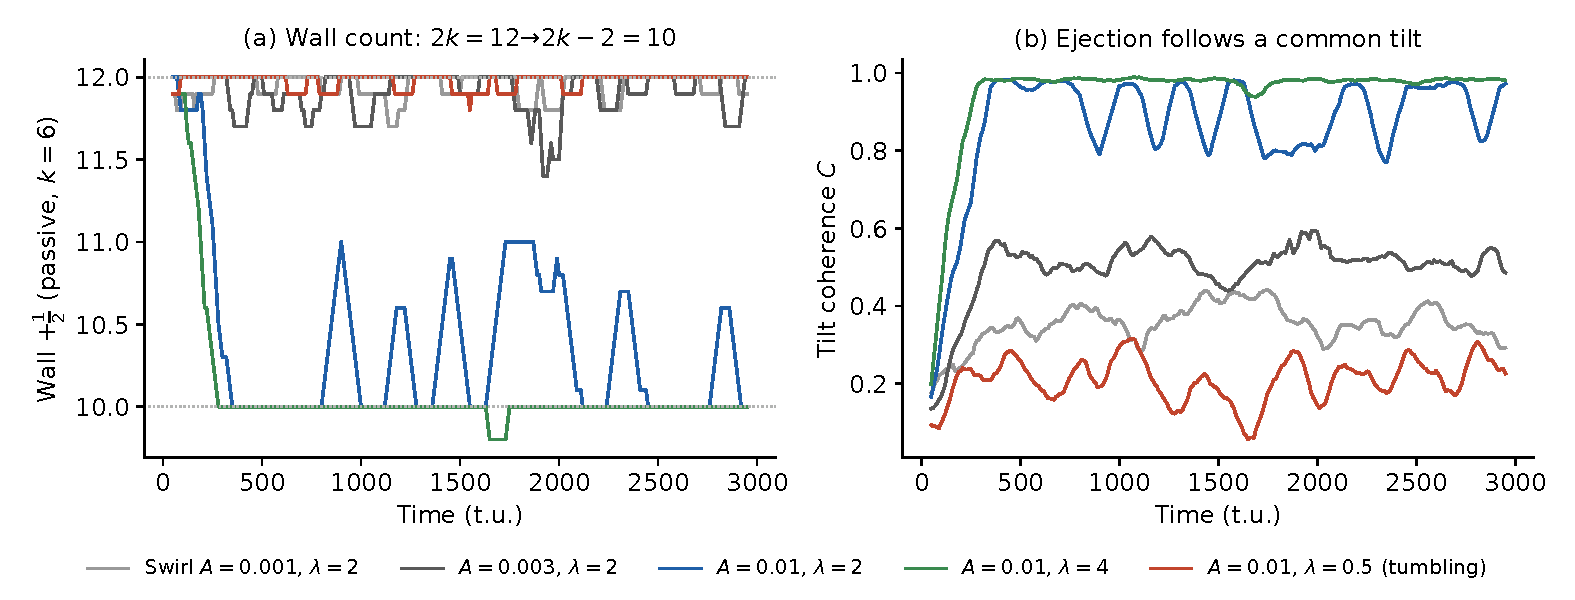
\includegraphics[width=\columnwidth]{fig_ejection}
\caption{\todo{Fig.~4}: passive cavity under an imposed vortex.}\label{fig:ejection}
\end{figure}

% ============================================================================================
\section{Where the flow comes from}\label{sec:hydro}
The bulk active stress drives the circulation; the wall layer opposes it and, seen from the bulk, acts as a planar winding-1 boundary whose tilt feeds back on the flow.
%% CONTENT: director-field Stokes (Fig. dirstokes: R^2 0.48-0.72; bulk drives incl. the two-vortex part; wall band opposes, common scale);
%% effective boundary (Fig. effective_bc: site pattern fades as e^{-2 pi delta/l}; spiral offset c = 90 + tau/2); linear stability -> onset R/l_a 0.4-0.6;
%% why point-defect models fail (SM). Could move largely to the SM if length is tight.

% ============================================================================================
\section{The tilt law}\label{sec:tilt}
The tilt is the flow-aligned angle in the no-slip shear next to the wall, $\tau=\arccos(1/\lambda)$, with no free parameter.
%% CONTENT: continuum test with the measured flow (Fig. shear_tilt); flat-wall theory: zero mode, leading order, boundary-layer correction (Fig. fig_flatwall);
%% mechanism in MPCD (director rotation at the defects' depth = Leslie angle, tilt = 2x);
%% active MPCD circles across lambda (Fig. fig_tiltlaw: within 3 deg for lambda 2-6, k 4/6/8); breakdown below lambda ~ 2 and its size dependence (runs/lamsize, TODO);
%% the last few degrees (residual +3 -> -2.5 deg with lambda; boundary layer absent in MPCD; order-dependent alignment; splay != bend) -> keep short, details in SM.
\begin{figure}[t]
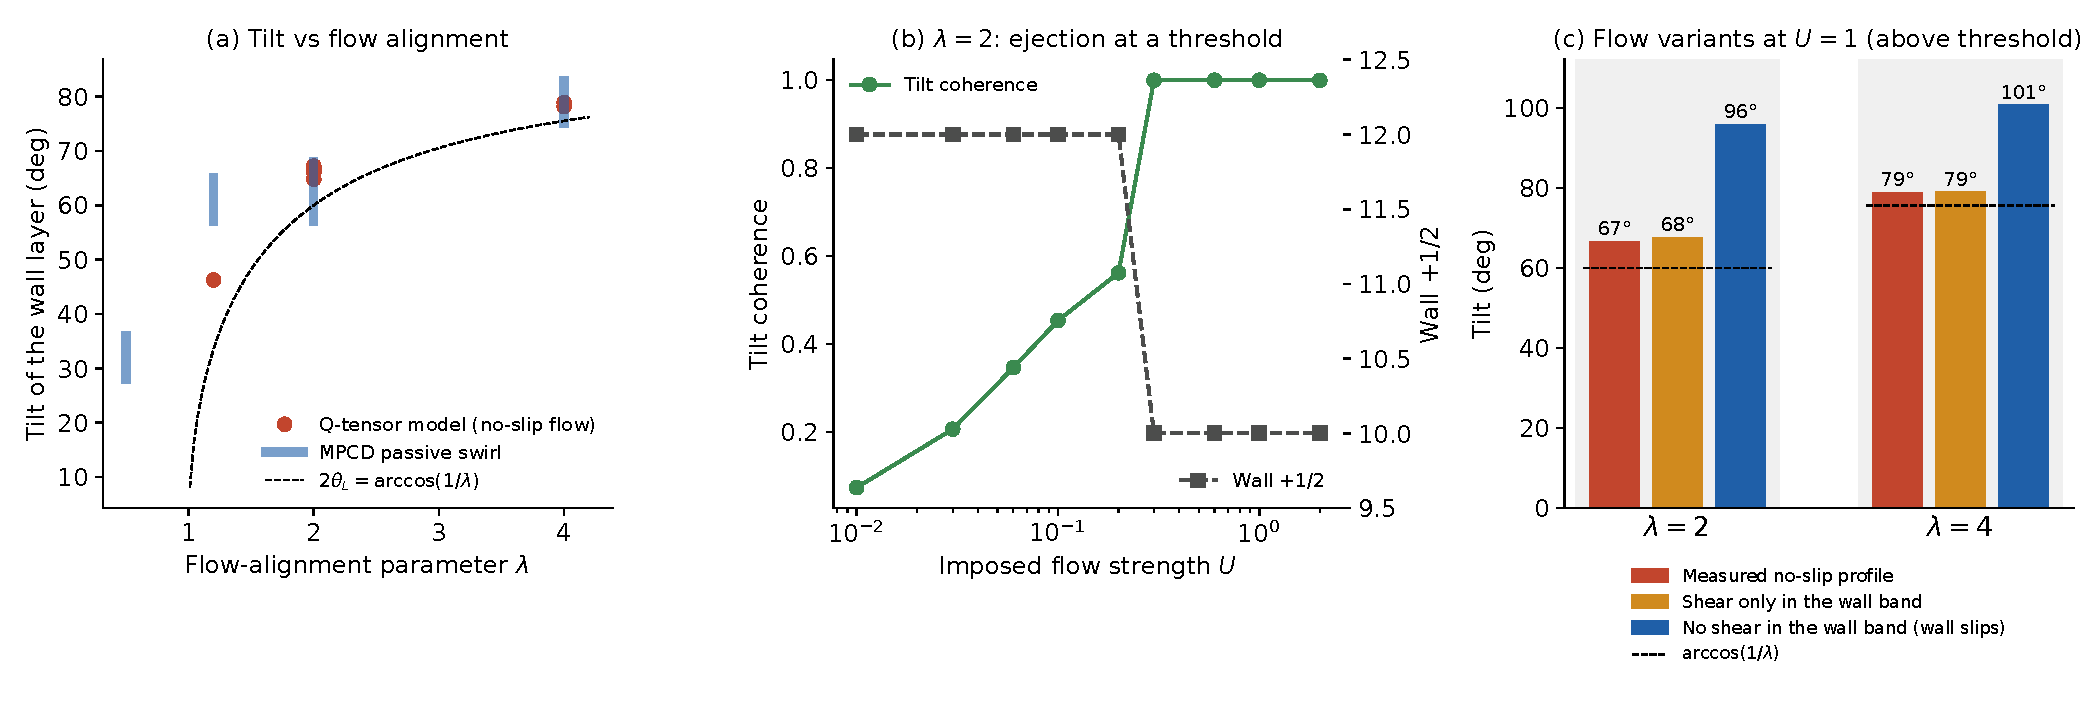
\includegraphics[width=\columnwidth]{shear_tilt}
\caption{\todo{Fig.~5}: Q-tensor model with the measured no-slip flow.}\label{fig:sheartilt}
\end{figure}
\begin{figure}[t]
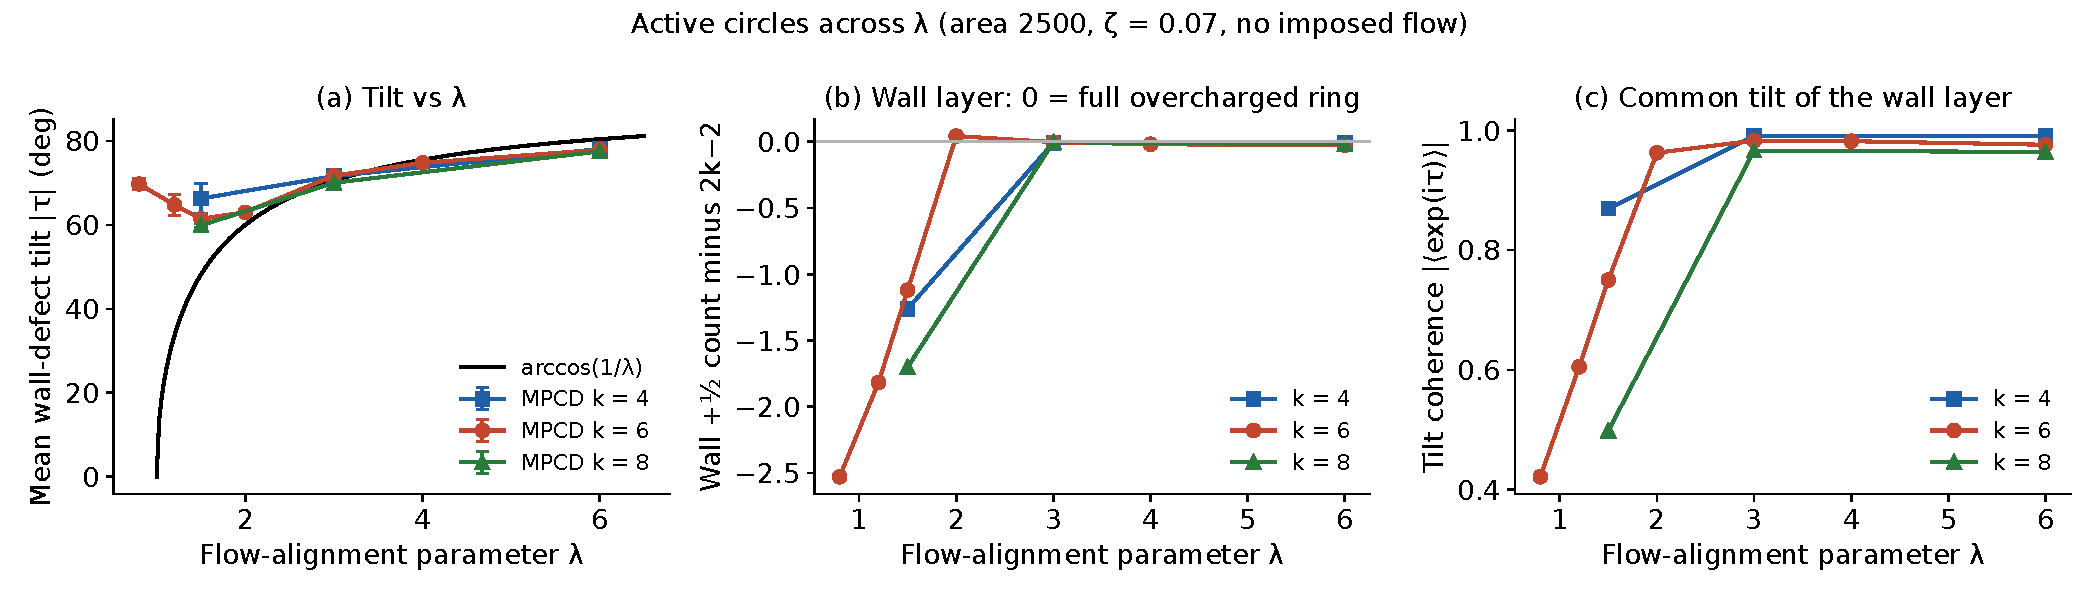
\includegraphics[width=\columnwidth]{fig_tiltlaw}
\caption{\todo{Fig.~6}: tilt law in active MPCD circles across $\lambda$ (with the flat-wall theory as an inset or in App.~A).}\label{fig:tiltlaw}
\end{figure}

% ============================================================================================
\section{Elongated cavities: loss of the coherent vortex}\label{sec:shapes}
Elongation beyond aspect ratio 1.25--1.37 breaks the single coherent vortex in ellipses and Cassini ovals alike, at every size, and the wall layer loses defects.
%% CONTENT: phase diagram (Fig. phase_shapes; scale-free transition); continuum reproduces it (Fig. fig_cont_ellipse);
%% layer loss is escape-driven, non-cascading, refill not starved (Fig. fig_shapes_mech); effective restoring force collapses (Fig. fig_restoring; elastic part unchanged);
%% elastic shielding (Fig. fig_shielding_layer; master Sec. shielding theory): exact in circles (shell theorem with same-sign images; passive depth law; screened approach),
%% ~9x weaker in an ideally filled ellipse (14 vs 1.6 kBT; 27 with the winding flux), lost with the measured depleted, unevenly spaced layer (interior tilted by ~180-230 kBT inside the 0.6 level towards the gaps; 7 evenly spaced: only 27) -> the leaky layer no longer screens the bulk;
%% bulk activity is the ingredient (activity only in the wall band keeps the coherent state; only in the bulk destroys it even in circles).
\begin{figure}[t]
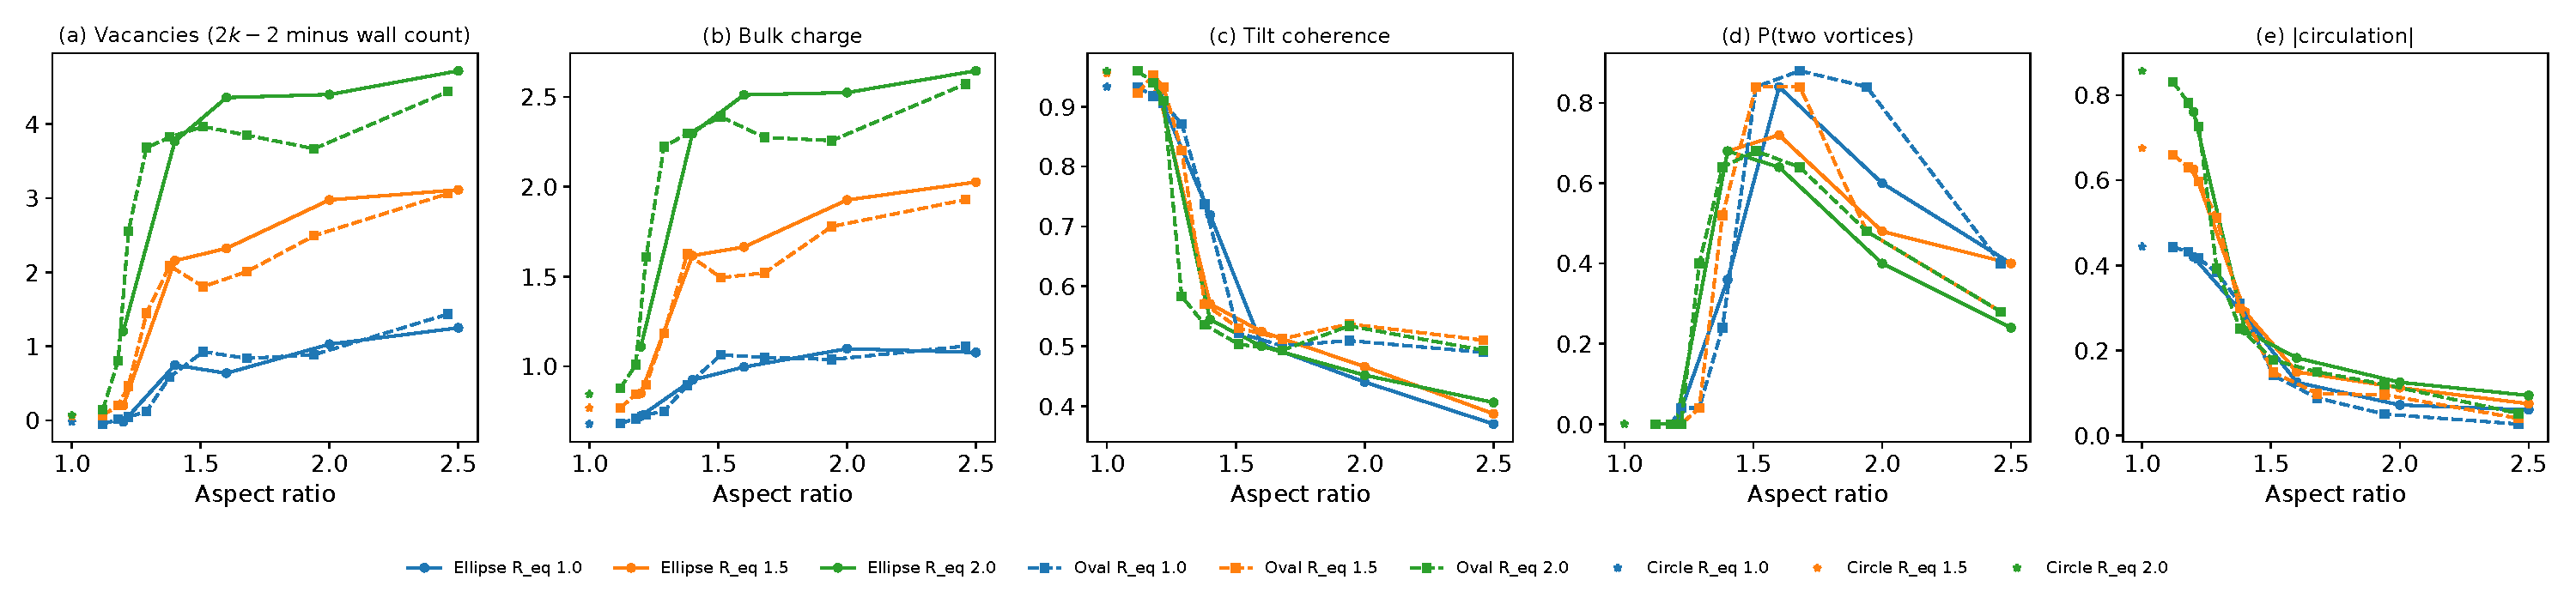
\includegraphics[width=\columnwidth]{phase_shapes}
\caption{\todo{Fig.~7}: shape sweep phase diagram.}\label{fig:phase}
\end{figure}
\begin{figure}[t]
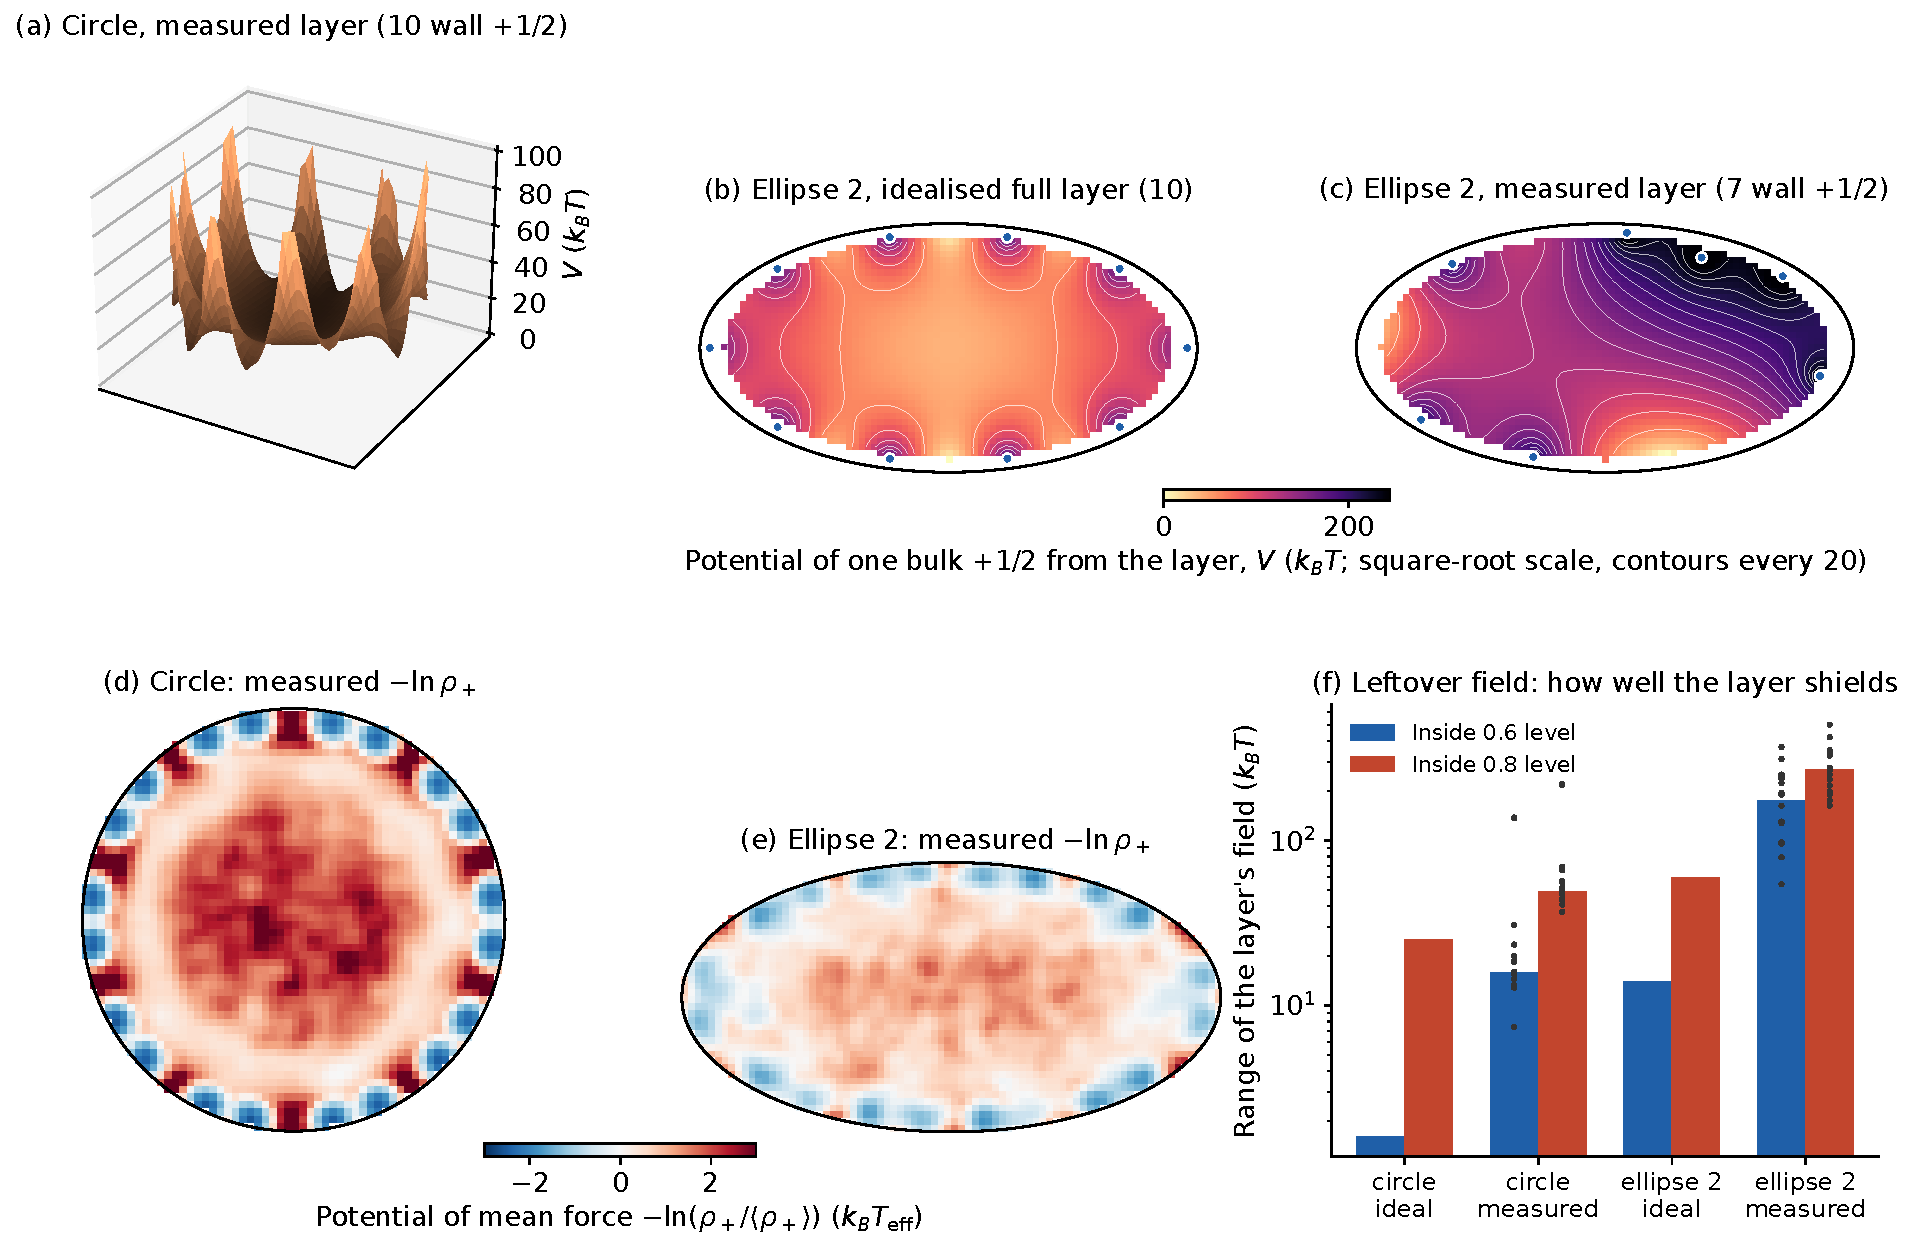
\includegraphics[width=\columnwidth]{fig_shielding_layer}
\caption{\todo{Fig.~7b}: elastic shielding by the wall layer, circle vs elongated (ideal and measured layers), and the measured potential of mean force.}\label{fig:shield}
\end{figure}

% ============================================================================================
\section{How a wall defect leaves}\label{sec:escape}
A wall $+\half$ is held mainly by its tilt and by the wall, not by elasticity: the tilt turns its active jet along the wall, and the no-slip wall transmits only a
third of the jet's inward component.
%% CONTENT: elastic barrier intact (Fig. fig_etsg_shapes); untilting run-up and own jet (Fig. fig_selfflow); wall blocks the normal component, g(d), closed law
%% 0.40 cos(tau) g(d) (Fig. fig_jetmap); wall-side lobe erased and recovering (Fig. fig_vortdef); landing on Q = 0 lines \cite{Head2024} (Fig. fig_qcrit);
%% force balance (alpha, beta, mu_n); tips vs flanks (Fig. fig_etsg_reg); ovals = ellipses; second, jet-free route with a passive wall band (Fig. fig_compare_bulk);
%% untilting is driven, not rotational diffusion (Langevin null model); precursors at -40 t.u. (closer wall neighbour, empty front). Several of these go to the SM.
\begin{figure}[t]
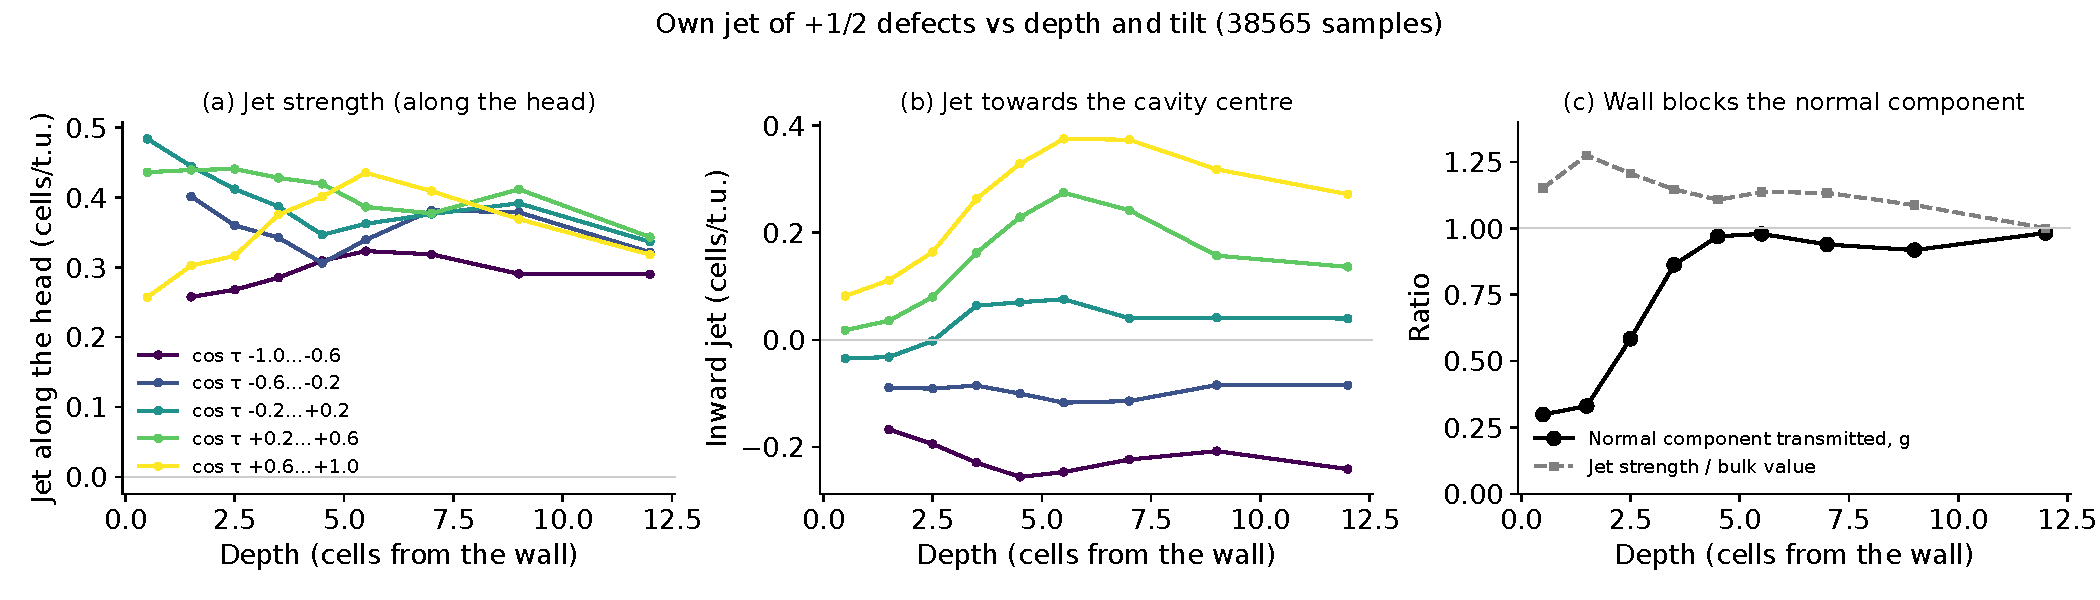
\includegraphics[width=\columnwidth]{fig_jetmap_ff12}
\caption{\todo{Fig.~8}: the wall blocks the inward component of a defect's own jet (composite with the untilting run-up and the lobe erasure).}\label{fig:jet}
\end{figure}

% ============================================================================================
\section{Mirror control: negative winding}\label{sec:mirror}
Reversing the winding puts $-\half$ defects, which are not self-propelled, in the wall layer. This tests whether the leak of elongated cavities is driven by the
wall defects' own active jets.
In the same 675 cavities as the $+k$ shape sweep (circles, ellipses, Cassini ovals; $R_\mathrm{eq}=1.0$, $1.5$, $2.0\,\la$; 3 seeds), the $-\half$ layer
holds where the $+\half$ layer leaks (Fig.~\ref{fig:mirror}). Medians over $k$, density and seeds, aspect $\geq1.4$: the $+\half$ layer loses 2.0 defects relative
to the circle (up to 4.7 at $R_\mathrm{eq}=2\,\la$) with an escape probability per wall defect of $0.017$ per 20\,t.u.; the $-\half$ layer loses $0.05$ with
$0.0006$ ($\approx30\times$ lower). In the largest elongated cavities the $-\half$ layer even gains (up to $0.9$ above the circle at $R_\mathrm{eq}=2\,\la$, aspect
2.5), and the bulk charge grows with it ($Q_b$ $0.8\to1.1$). The circulation collapses in both cases ($0.86\to0.09$ for $+k$, $0.66\to0.11$ for $-k$ at
$R_\mathrm{eq}=2\,\la$), so the loss of the coherent vortex alone does not empty the layer: the leak requires self-propelled wall defects, consistent with the
escape route of Sec.~\ref{sec:shapes}. In circles the $-\half$ layer gains about 1.5 of the two defects predicted by the continuum (13.5 of 14 within 4 cells of the wall
at $R\approx1.25\,\la$ for $k=-6$, fewer in larger circles at the same $k$; 13.0 at aspect 2 from seeded starts, unique from 12 and 14), with bulk charge $+0.5$ to $+0.7$.
The gain is set by crowding: in the sweep circles it reaches the full 2 for wall densities $\rho\gtrsim0.09$ at $R_\mathrm{eq}\geq1.5\,\la$ ($1.8$--$2.1$; 2.0 at $R_\mathrm{eq}=2\,\la$), and is
$0.1$--$0.3$ for the sparsest walls at $R_\mathrm{eq}\geq1.5\,\la$. The shortfall at intermediate crowding relative to the continuum is open. Wall $-\half$ also keep a restoring force in active ellipses ($k=-6$, 2 seeds: $-1.8$ to $-2.1$ at 2.5--3 cells; passive, aspect 2: $-2.6$).
\begin{figure*}[t]
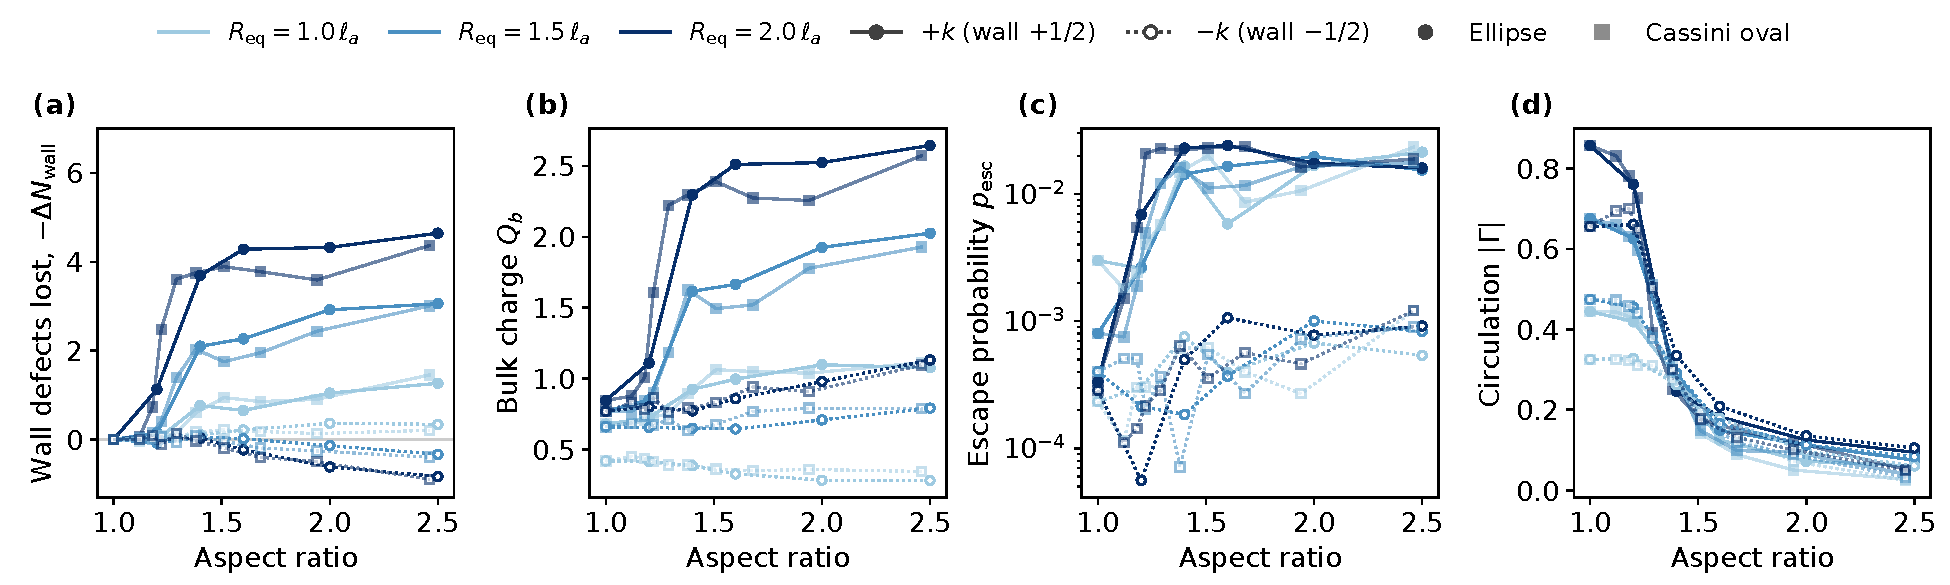
\includegraphics[width=\textwidth]{fig_mirror_shapes}
\caption{Mirror control: $+k$ (wall $+\half$, solid) vs $-k$ (wall $-\half$, dotted) in the same cavities against aspect ratio (ellipses, ovals; three sizes; medians
over $k$, density, 3 seeds). (a) Wall defects lost relative to the circle. (b) Bulk charge. (c) Escape probability per wall defect per 20\,t.u. (d) $|$Circulation$|$.}\label{fig:mirror}
\end{figure*}

% ============================================================================================
\section{The steady state and the wall law}\label{sec:steady}
\subsection{Rates are set by the tilt, the population by a balance}
%% CONTENT: lambda test in the aspect-2 ellipse (escapes 10x fewer from lambda 2 to 4, refills slowed too: exits 6x, entries 3.7x; wall count 7.1 -> 7.65);
%% depleted layer is far above the elastic optimum (refill lowers the Frank energy by 80-100 kBT); unique steady state from seeded starts (4/7/10 -> 7.2);
%% self-limitation by layer crowding (exit rate 0.068 -> 0.028 per 20 t.u. with 0 -> 5 vacancies).
\subsection{A wall law}
%% CONTENT: Fig. fig_perlength: bulk charge per unit wall length saturates by aspect 1.5, set by q = k/P (c ~ 0.012 at q 0.03; released fraction 0.61 -> 0.10; provenance/perlength_qbins.txt);
%% Q_b ~ c(q) P (area^0.47 at fixed q); circles exactly +1 (topologically protected).
\subsection{The flat limit: a winding channel}
%% CONTENT (keep to one paragraph + one figure or SM figure, per scope): periodic channel with opposite windings, same released share (41-43 %) at W 20-60,
%% down to W ~ 18 (narrow-channel runs 2026-10-14; W 12-14 break down, one seed locks into coherent flow). Fig. fig_channel (or SM).
\begin{figure}[t]
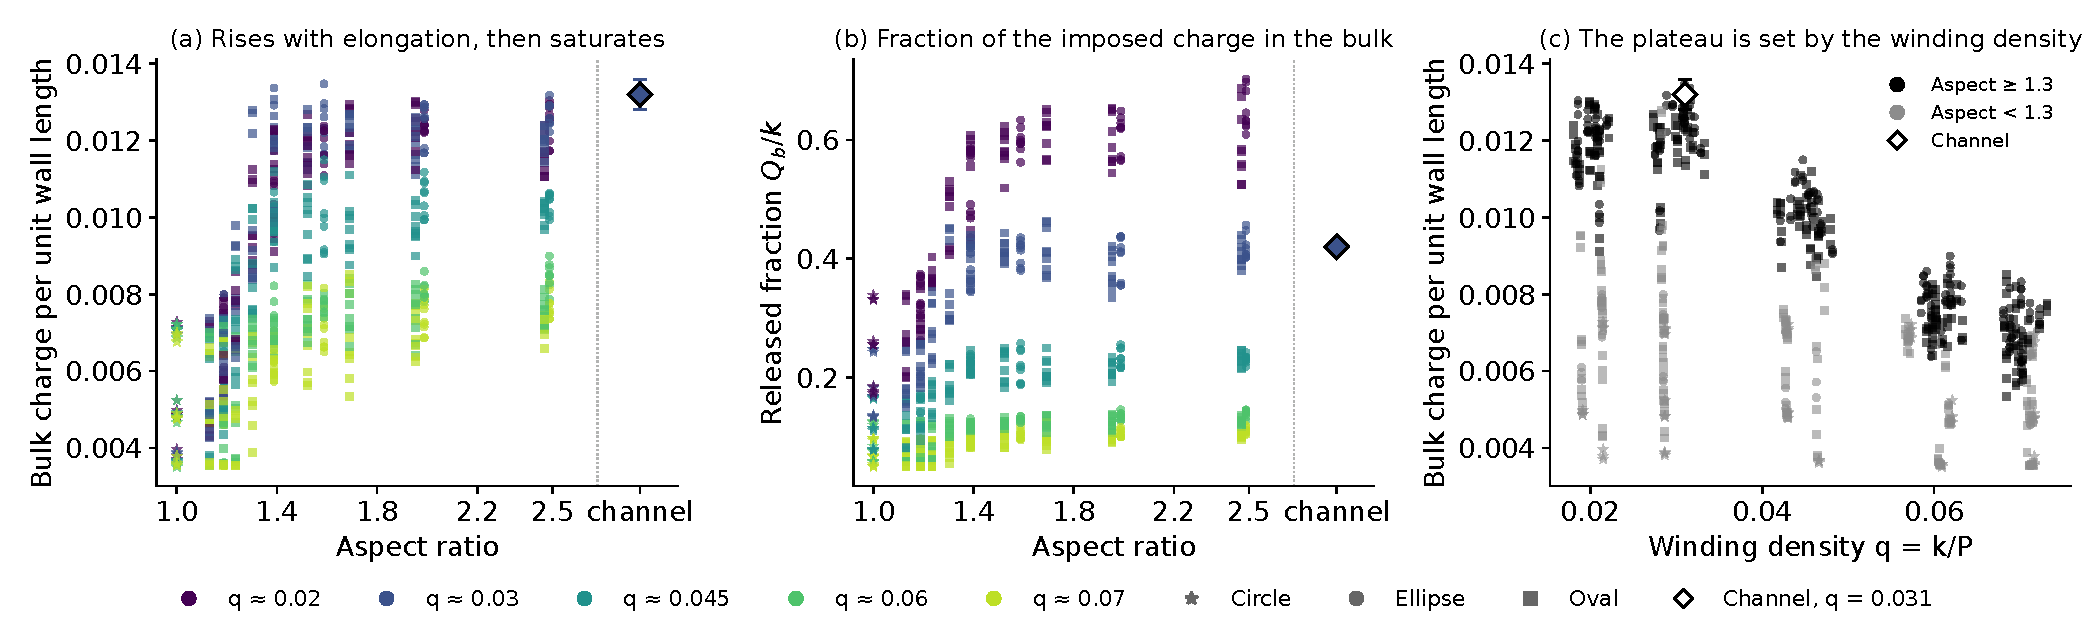
\includegraphics[width=\columnwidth]{fig_perlength}
\caption{\todo{Fig.~9}: the wall law.}\label{fig:walllaw}
\end{figure}

% ============================================================================================
\section{Discussion}\label{sec:discussion}
%% CONTENT: what is universal (flow-aligning active nematic + patterned anchoring; tilt law with no free parameter; wall law); experimental proposal
%% (microtubule-kinesin or epithelial layers in wells with patterned winding; predicted tilt arccos(1/lambda) and bulk charge); open questions:
%% negative winding in MPCD vs continuum, onset k-ordering, the trigger of untilting, the residual tilt trend; outlook: channels and the 'topological capacitor' (paper 2/3).
\todo{discussion}

% ============================================================================================
\appendix
\section{Flat-wall theory}\label{app:flatwall}
%% CONTENT: Ericksen-Leslie with the winding anchoring; zero mode; leading order arccos(1/lambda); boundary-layer correction Eq. and its test (Fig. fig_flatwall).
\section{Layer versus bulk defects}\label{app:layer}
%% CONTENT: 4-cell criterion; depth distribution, mobility crossover, weak site locking (Fig. fig_layer_profile).
\section{Methods details}\label{app:methods}
%% CONTENT: MPCD parameters; Frank constants and gamma_1; active length; defect tracking; escape detection and controls; Fokker-Planck construction;
%% elastic point-defect model (anisotropic, relaxed cores; Cassini walls); director-field Stokes; Q-criterion and smoothing.
%% Supplementary material (separate file): movies (escape events with lobe overlay), fluctuation theory, half-integer k, negative-layer energetics,
%% point-defect model failures, interval statistics, precursor and Langevin analyses, ovals in detail, lambda breakdown details.

\bibliography{../refs}
\end{document}
